\section{Przegląd metod segmentacji obrazu}
\subsection{Wstęp}
Segmentacja obrazu jest procesem umożliwiającym podział obrazu na obszary, które pod względem zadanego kryterium różnią się miedzy sobą. W zależności od kryterium, podczas procesu segmentacji można wyodrębnić z obrazu obiekty posiadające określone kształty, kolory czy rozmiar. W wyniku segmentacji obrazu, uzyskujemy obraz, który nie zawiera zbędnych (z punktu widzenia dalszego przetwarzania) szczegółów.\\
Przykładem zastosowania metod segmentacji obrazów może być problem liczenia wbitych gwoździ do elementu na taśmie produkcyjnej. Obraz wejściowy (przedstawiony na rysunku~\ref{fig:gwozdzie_input}) ze względu na różnorodne tło i jasność elementów, trudno przeanalizować pod kątem liczenia obiektów. Natomiast ten sam obraz poddany operacji segmentacji (rysunek~\ref{fig:gwozdzie_output}) zawiera w sobie tylko i wyłącznie elementy, które są interesujące z punktu widzenia problemu jaki trzeba rozwiązać. Na podstawie koloru oraz kształtu możliwe było wyeliminowanie obiektów, które nie były istotne w danym zadaniu.

\begin{figure}
  \centering
  \begin{subfigure}[b]{0.48\textwidth}
    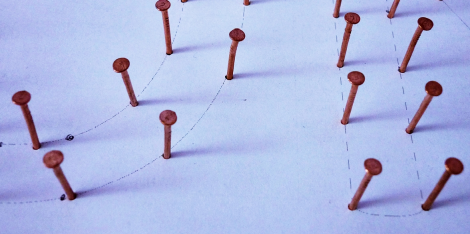
\includegraphics[width=\textwidth]{img/gwozdzie-input}
    \caption{Obraz wejściowy}
    \label{fig:gwozdzie_input}
  \end{subfigure}
  ~
  \begin{subfigure}[b]{0.48\textwidth}
    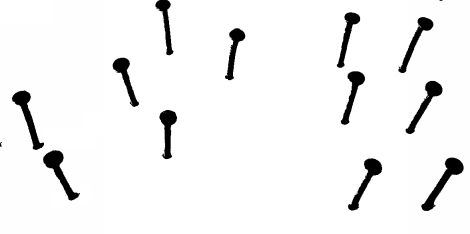
\includegraphics[width=\textwidth]{img/gwozdzie-output}
    \caption{Obraz po operacji segmentacji}
    \label{fig:gwozdzie_output}
  \end{subfigure}
  \caption{Przykład zastosowania metody segmentacji obrazu}\label{fig:gwozdzie}
\end{figure}

\subsection{Progowanie}
Najłatwiejszą metodą segmentacji obrazu jest metoda progowania, opisywana w podrozdziale \nameref{sssec:threshold}.

\subsection{Detekcja krawędzi}
Celem algorytmów detekcji krawędzi jest znalezienie na obrazie zbioru punktów, które reprezentują obrysy poszukiwanych elementów. 

\subsubsection{Algorytm Robertsa}
Algorytm Robertsa do wykrywania krawędzi w obrazie jest jednym z pierwszych algorytmów w swojej kategorii. Cechuje się szybkością działania oraz stosunkowo niską odpornością na szumy. Działanie algorytmu wymaga zastosowaniu dla każdego piksela obrazu dwóch masek:
\begin{gather*}
  M_x = \begin{matrix}
    \begin{bmatrix}
      +1 & 0 \\
      0 & -1
    \end{bmatrix}
    &
    M_y = \begin{bmatrix}
      0 & +1 \\
      -1 & 0
    \end{bmatrix}
  \end{matrix}
\end{gather*}
Zdefiniujemy funkcje pomocnicze $f_x$ oraz $f_y$:
\begin{gather*}
  f_x(x, y) = M_x[0][0] \cdot f^{(in)}(x, y) + M_x[0][1] \cdot f^{(in)}(x+1, y) +\\ \quad\quad\quad\quad\quad\quad M_x[1][0] \cdot f^{(in)}(x, y+1) + M_x[1][1] \cdot f^{(in)}(x+1, y+1) \\
  f_x(x, y) = M_y[0][0] \cdot f^{(in)}(x, y) + M_y[0][1] \cdot f^{(in)}(x+1, y) +\\ \quad\quad\quad\quad\quad\quad M_y[1][0] \cdot f^{(in)}(x, y+1) + M_y[1][1] \cdot f^{(in)}(x+1, y+1)
\end{gather*}
Wartość jasności poszczególnych pikseli obrazu wyjściowego wyliczane są następującym wzorem:
\begin{gather*}
  f^{(out)}(x, y) = \sqrt{f_x^2(x, y)+f_{y}^2(x, y)}.
\end{gather*}
Kierunek gradientu może zostać wyznaczony ze wzoru:
\begin{gather*}
  \theta(x, y) = arctan(\frac{f_{y}(x, y)}{f_{x}(x, y)}).
\end{gather*}
\subsubsection{Sobel} \label{sssec:sobel}
Algorytmu Sobel jest bardzo podobny do przedstawionego wcześniej algorytmu Robertsa. W przypadku tego algorytmu, dane są dwie maski o następującej postaci:
\begin{gather*}
\begin{matrix}
  M_x = \begin{bmatrix}
    -1 & 0 & +1 \\
    -2 & 0 & +2 \\
    -1 & 0 & +1
  \end{bmatrix}
&
  M_y = \begin{bmatrix}
    -1 & -2 & -1 \\
    0 & 0 & 0 \\
    +1 & +2 & +1
  \end{bmatrix}
\end{matrix}
\end{gather*}
Zdefiniujemy dwie funkcje pomocnicze $f_x$ oraz $f_y$:
\begin{gather*}
  f_x  = M_x * f^{(in)}, \\
  f_y  = M_y * f^{(in)}.
\end{gather*}
Funkcję jasności obrazu wyjściowego możemy zdefiniować następująco:
\begin{gather*}
  f^{(out)}(x, y) = \sqrt{f_x^2(x, y)+f_{y}^2(x, y)}.
\end{gather*}
Algorytm jest znacznie bardziej odporny na szumy występujące na obrazie niż algorytm Robertsa. \\
Kierunek gradientu może zostać wyznaczony za pomocą wzoru:
\begin{gather*}
  \theta(x, y) = arctan(\frac{f_y(x, y)}{f_x(x, y)}).
\end{gather*}
\subsubsection{Algorytm Canny'ego}
Algorytm Canny'ego składa się z czterech podstawowych kroków.
\begin{enumerate}
\item Wygładzanie obrazu \\
  Celem tego kroku jest usunięcie z obrazu szumów mogących wystąpić na obrazie. Szumy mogą powodować detekcję fałszywych krawędzi, dlatego usunięcie ich przed faktycznym procesem wyszukiwania algorytmu powoduje poprawę jakości wyników algorytmu. W algorytmie Canny'ego do wygładzenia obrazu stosuje się filtr Gaussa. 
\item Znajdowanie gradientu \\
  Do znajdowania gradientu obrazu wykorzystywany jest operator sobela, opisywany w podrozdziale \nameref{sssec:sobel}.
\item Tłumienie nie-maksymalnych sygnałów \\
  Po zastosowaniu operatora Sobel, krawędzie obrazu są rozmyte. W tym kroku następuje filtrowanie wszystkich lokalnych maksymalnych wartości w obrazie gradientowym, oraz usunięcie wartości nie-maksymalnych. Dla każdego piksela, kierunek gradientu zaokrąglany jest z dokładnością do 45 stopni, otrzymując w ten sposób 8 wartości kierunków. Dla każdego piksela pod uwagę brane są trzy wartości: wartość badanego piksela, najbliższy piksel wskazywany przez kierunek gradientu, oraz najbliższy piksel leżący w przeciwnym kierunku niż kierunek wskazywany przez gradient. Jeśli badany piksel ma wartość maksymalną spośród trzech podanych wartości, nie zostaje on usunięty. W przeciwnym razie, wartość piksela zostaje zastąpiona wartością zerową.
\item Podwójne progowanie(progowanie z histerezą)
  Pomimo zastosowania metody wygładzania w pierwszym etapie algorytmu, znalezienie niektórych krawędzi może być efektem zaszumionego obrazu. Dlatego w algorytmie Canny'ego stosuje się podwójne progowanie, z wartościami:
$T_{high}$ - wartość wyższego progu,\\
$T_{low}$ - wartość niższego progu,\\
będącymi w relacji:
\begin{gather*}
  T_{max} \geq T_{min} 
\end{gather*}.
Piksele o wartościach większych niż $T_{high}$ klasyfikowane są jako \textit{krawędzie silne}. Piksele o wartościach pomiędzy $T_{low}$ i $T_{low}$ to tzw. \textit{krawędzie słabe}. Piksele o wartościach mniejszych niż $T_{min}$ są usuwane z obrazu.

\end{enumerate}

\subsection{Algorytmy wykorzystujące histogram}
Algorytmy wykorzystujące analizę histogramu obrazu cechuje szybkość działania, ponieważ budowa histogramu wymaga tylko jednej iteracji przez wszystkie piksele w obrazie. Istnieje kilka technik segmentacji obrazu w oparciu o analizę histogramu. \\
Przed wykonaniem jednego z niżej omawianych algorytmów, w celu poprawy rezultatów, należy zastosować operację wyrównania histogramu, oraz operację wygładzenia histogramu.

\subsubsection{Wyszukiwanie szczytów histogramu}
Wyszukiwanie szczytów histogramu wykorzystywane jest do separacji tła od obiektu pierwszoplanowego. Po wyznaczeniu histogramu, wyszukiwane zostają dwa maksimum lokalne, posiadające największe wartości (są to tzw. wartości szczytowe). Następnie na podstawie tych wartości wyznaczana jest progowa wartość, służąca do klasyfikacji pikseli na obrazie:
\begin{gather*}
  T = \frac{p_1 + p_2}{2},
\end{gather*}
gdzie $p_1$ jest pierwszą wartością szczytową w histogramie, a $p_2$ jest drugą wartością szczytową w histogramie. \\
W rzeczywistych przypadkach bardzo często występuje sytuacja, w której piksele tła oraz piksele obiektu pierwszoplanowego nie mają takich samych wartości dla całego obiektu, ale przyjmują wiele wartości oscylujących wokół jednej z nich. Przykład takiego obrazu został pokazany na rysunku~\ref{fig:histogram_peaks}. Histogram zawiera widoczne trzy skupiska wartości(na pozycjach: 8, 18 oraz 44), natomiast obydwie największe wartości szczytowe w histogramie należą do jednego skupiska. Aby wyeliminować ten problem, należy zdefiniować minimalną odległość pomiędzy szczytami histogramu. Jeśli drugi szczyt będzie znajdował się zbyt blisko pierwszego, należy go odrzucić, i rozpocząć poszukiwanie kolejnego szczytu. Nie uwzględniając minimalnego odstępu pomiędzy szczytami, do wyznaczenia progu zostały by wybrane liczby 8 oraz 18, ponieważ są to dwie największe wartości w histogramie. Obydwie te wartości reprezentują tło, przez co segmentacja się nie powiodła (co można zobaczyć na rysunku~\ref{fig:histogram_peaks_bad}. Jeśli założymy, że szczyty nie mogą znajdować się o wartość \frac{1}{3} szerokości histogramu, do wyznaczenia progu zostanie użyta wartość 8 oraz 44. Wynikiem segmentacji natomiast będzie obraz przedstawiony na rysunku~\ref{fig:histogram_peaks_good}. Zwykle wartość minimalnej odległości pomiędzy szczytami dobiera się na podstawie przeprowadzonych wcześniej badań na danych testowych.
\begin{figure}
  \centering
  \begin{subfigure}[b]{0.7\textwidth}
    
\includegraphics[width=\textwidth]{img/histogram-peaks-input}
    \caption{Obraz wejściowy}
    \label{fig:histogram_peaks_input}
  \end{subfigure}
  ~
  \begin{subfigure}[b]{0.7\textwidth}
    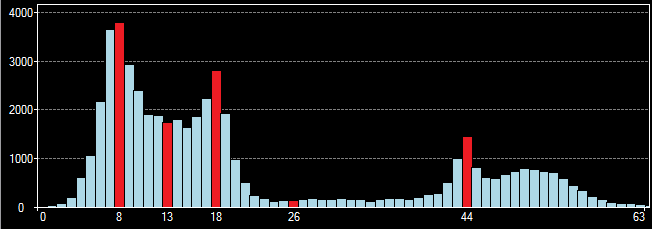
\includegraphics[width=\textwidth]{img/histogram-peaks-histogram}
    \caption{Histogram obrazu wejściowego}
    \label{fig:histogram_peaks_histogram}
  \end{subfigure}
  ~
  \begin{subfigure}[b]{0.45\textwidth}
    
\includegraphics[width=\textwidth]{img/histogram-peaks-bad}
    \caption{Obraz po operacji progowania, wartość progu: 13}
    \label{fig:histogram_peaks_bad}
  \end{subfigure}
  ~
  \begin{subfigure}[b]{0.45\textwidth}
    
\includegraphics[width=\textwidth]{img/histogram-peaks-good}
    \caption{Obraz po operacji progowania, wartość progu: 26}
    \label{fig:hitogram_peaks_good}
  \end{subfigure}
  \caption{Progowanie przez wyszukiwanie szczytów histogramu}\label{fig:histogram_peaks}
\end{figure}

\subsubsection{Wyszukiwanie minimum histogramu}
Metoda wyszukiwania minimum histogramu jest bardzo podobna do metody omawianej w poprzednim podpunkcie. Na początku wyszukiwane są dwie wartości szczytowe, które powinny być odległe od siebie o pewną ustaloną wartość. Jednak w przeciwieństwie do omawianego wcześniej algorytmu, jako wartość progową przyjmuje się najmniejszą wartość pomiędzy dwoma szczytami w histogramie. \\
Rysunek~\ref{fig:histogram_valleys} przedstawia histogram pewnego obrazu. Stosując metodę wyszukiwania szczytów histogramu, jako wartość progowa wybralibyśmy wartość 102 (szczyty histogramów znajdują się na pozycjach 48 i 155). Stosując omawianą w tym akapicie metodę, jako wartość progowa zostanie wybrana wartość 129, która jest minimalną wartością znajdującą się pomiędzy szczytami histogramu.

\begin{figure}
  \centering
  \begin{subfigure}[b]{0.7\textwidth}
    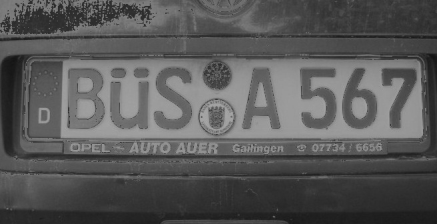
\includegraphics[width=\textwidth]{img/histogram-valleys-input}
    \caption{Obraz wejściowy}
    \label{fig:histogram_valleys_input}
  \end{subfigure}
  ~
  \begin{subfigure}[b]{0.7\textwidth}
    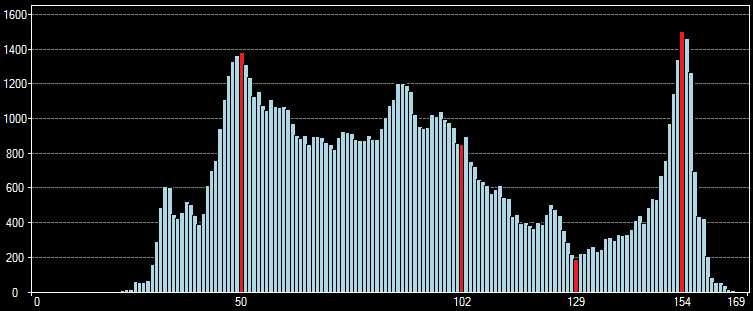
\includegraphics[width=\textwidth]{img/histogram-valleys-histogram}
    \caption{Histogram obrazu wejściowego}
    \label{fig:histogram_valleys_histogram}
  \end{subfigure}
  ~
  \begin{subfigure}[b]{0.45\textwidth}
    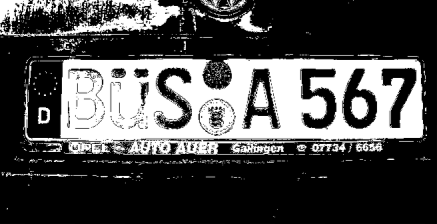
\includegraphics[width=\textwidth]{img/histogram-valleys-bad}
    \caption{Obraz po operacji progowania, wartość progu: 102}
    \label{fig:histogram_valleys_bad}
  \end{subfigure}
  ~
  \begin{subfigure}[b]{0.45\textwidth}
    
\includegraphics[width=\textwidth]{img/histogram-valleys-good}
    \caption{Obraz po operacji progowania, wartość progu: 129}
    \label{fig:hitogram_valleys_good}
  \end{subfigure}
  \caption{Progowanie przez wyszukiwanie minimum pomiędzy szczytami histogramu}\label{fig:histogram_valleys}
\end{figure}
\subsection{Segmentacja przez rozrost obszarów}
Metoda segmentacji przez rozrost obszarów polega na wyszukiwanie na obrazie elementów o podobnej jasności. Algorytm rozpoczyna działanie od punktów startowych, które powinny zostać podane jako parametr algorytmu. Algorytm można opisać w następujący sposób:
\begin{enumerate}
  \item Nadaj każdemu punktowi startowemu etykietę.
  \item Dodaj punkty startowe do kolejki.
  \item Jeśli kolejka jest pusta, zakończ algorytm.
  \item Pobierz punkt z kolejki, a następnie sprawdź wszystkie punkty znajdujące się w sąsiedztwie pod względem podobieństwa. Jeśli sąsiedni punkt spełnia kryterium podobieństwa, oznacz go etykietą punktu pobranego z kolejki, a następnie umieść punkt w kolejce.
  \item Przejdź do kroku 3.
\end{enumerate}
Wynikiem algorytmu będzie zbiór punktów oznaczonych etykietami. Punkty oznaczone tą samą etykietą reprezentują pojedynczy obszar znaleziony na obrazie.

Podczas projektowania metody segmentacji przez rozrost, należy, biorąc pod uwagę warunki działania algorytmu, rozważyć dwa problemy:
\begin{itemize}
  \item wybór punktów startowych,
  \item wybór kryterium podobieństwa
\end{itemize}.
W celu rozwiązania pierwszego problemu, można zastosować jedną z wcześniej omawianych metod segmentacji (np. szybki algorytm progowania), a następnie wybrać punkty oddalone od siebie o zadaną wartość. \\
Kryterium podobieństwa może zostać określone na dwa sposoby, w zależności od problemu, do rozwiązywania którego został zaprojektowany algorytm:
\begin{enumerate}
  \item dla obrazów w których różnica jasności w ramach jednego obszaru może być bardzo duża, należy zastosować kryterium 
    \begin{gather*}
      |f^{(in)}(p_x, p_y) - f^{(in)}(n_x, n_y)| < \varepsilon,
    \end{gather*}
    gdzie $p_x$ oraz $p_y$ to współrzędne aktualnie przetwarzanego punktu, $n_x$ i $n_y$ to współrzędne aktualnie przetwarzanego sąsiada, a $\varepsilon$ to maksymalna różnica jasności pomiędzy sąsiednimi punktami, taka, że dwa punkty uznawane są za przynależne do tego samego obiektu. Stosując powyższe kryterium mamy pewność, że obiekt ze zmiennym natężeniem oświetlenia zostanie sklasyfikowany jako jeden obszar. Stosowanie tego kryterium może jednak spowodować, że do obszaru zostaną zaklasyfikowane elementy tła.
    \item dla obrazów o stałym oświetleniu, stosuje się kryterium
      \begin{gather*}
        |f^{(in)}(seed_x, seed_y) - f^{(in)}(n_x, n_y)| < \varepsilon
      \end{gather*}
      gdzie $seed_x$ i $seed_y$ to współrzędne punktu wejściowego. Stosując powyższe kryterium mamy pewność, że obiekt ze zmiennym natężeniem oświetlenia zostanie sklasyfikowany jako jeden obszar. Stosowanie tego kryterium może jednak spowodować, że do obszaru zostaną zaklasyfikowane elementy tła.
\end{enumerate}
Na rysunku~\ref{fig:region_growing} przedstawiony został wynik operacji segmentacji obrazu przez rozrost obszarów stosując dwa różne kryteria.
\begin{figure}
  \centering
  \begin{subfigure}[b]{0.45\textwidth}
    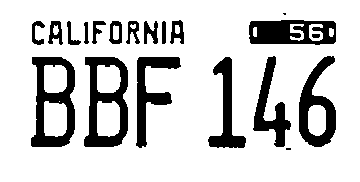
\includegraphics[width=\textwidth]{img/region-growing-relative}
    \caption{Obraz wynikowy dla kryterium 1)}
    \label{fig:region_growing_relative}
  \end{subfigure}
  ~
  \begin{subfigure}[b]{0.45\textwidth}
    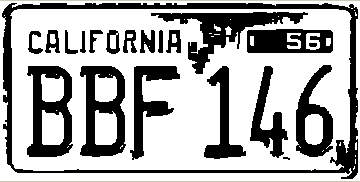
\includegraphics[width=\textwidth]{img/region-growing-absolute}
    \caption{Obraz wynikowy dla kryterium 2)}
    \label{fig:region_growing_absolute}
  \end{subfigure}
  \caption{Porównanie wyników uruchomienia algorytmu rozrostu obszarów z zastosowaniem różnych kryterium}
    \label{fig:region_growing}
\end{figure}

\subsection{Segmentacja przy użyciu rzutu jasności} \nameref{ssection:rzut_jasnosci}
Algorytm rzutu jasności bardzo dobrze sprawdza się w lokalizacji obiektów na obrazie, kiedy natężenie koloru obiektu znacząco różni się od koloru tła, a ponadto, obiekty zajmują znaczącą część powierzchni obrazu. Obraz rozpatrywany jest zarówno w poziomie, jak i w pionie. Dla każdego wiersza(kolumny) w obrazie, sumuje się wszystkie wartości pikseli należące dla danego wiersza(kolumny), otrzymując tablicę wartości:
\begin{gather*}
  G_x[i] = \sum\limits_{i=1}^M f^{(in)}(i, j) \; dla \; i = 0,1,2,...,M, \\
  G_y[j] = \sum\limits_{j=1}^N f^{(in)}(i, j) \; dla \; j = 0,1,2,...,N,
\end{gather*} gdzie $P_x$ oraz $P_y$ to tablice rzutu jasności. Analizując tablice rzutu jasności można zauważyć, że w miejscach na obrazie, gdzie występują obiekty, wartości w tablicy przyjmują wartości znacznie większe w przypadku, gdy kolor tła jest ciemniejszy od obiektu, lub znacznie mniejsze, w przypadku gdy kolor tła jest jaśniejszy od obiektu. Na podstawie tych informacji możliwe jest zlokalizowanie obiektów na obrazie. Rysunek~\ref{fig:rzut_jasnosci} przedstawia użycie metody segmentacji przy użyciu rzutu jasności dla przykładowej tablicy rejestracyjnej. Tablice rzutu jasności przedstawione zostały w postaci histogramu. W miejscach, gdzie pojawiają się na obrazie litery, wartości histogramu są mniejsze.

\begin{figure}
  \centering
  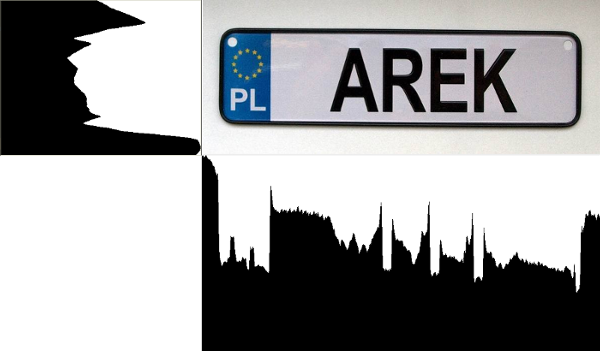
\includegraphics[width=15cm]{img/rzut-jasnosci}
  \caption{Histogramy dla obrazu wygenerowane przez algorytm rzutu jasności dla przykładowego obrazu}
  \label{fig:rzut_jasnosci}
\end{figure}
\subsection{Metoda Sauvola i Pietikainena}
Algorytm polega na znalezieniu progu dla każdego piksela, analizując jego najbliższe otoczenia. Otoczenie rozumiemy przez zbiór pikseli które znajdują się w zdefiniowanym obszarze, a piksel, dla którego w danym momencie wyznaczana jest wartość progu, znajduje się na środku tego obszaru. Wartość progu wyznaczana jest według wzoru:
\begin{gather*}
  T(x, y) = \mu(x, y)\Big[1+k\big(\frac{\sigma(x, y)}{R} - 1\big)\Big], \quad k > 0,
\end{gather*}
gdzie:
T(x, y) - wartość progu dla piksela o współrzędnych (x, y),\\
$\mu$(x, y) - średnia wartości pikseli w zadanym otoczeniu piksela,\\
$\sigma(x, y)$ - odchylenie standardowe w zadanym otoczeniu piksela,\\
R - maksymalna wartość odchylenia standardowego(dla obrazu 8-bitowego jest to wartość 128),\\
k - parametr algorytmu. \\
\subsection{Segmentacja wododziałowa}
Algorytm segmentacji wododziałowej polega na odnajdowaniu na obrazie krawędzi, będących granicami szukanych segmentów. Segmentacja wododziałowa wzorowana jest na naturalnym procesie hydrologicznym, polegającym na tworzeniu się zlewisk w lokalnie najniżej położonych obszarach geograficznych. \\
\subsubsection{Podstawowe pojęcia}
Algorytm zostanie opisany używając terminologii występującej w geografii. Poniżej znajduje się rozwinięcie podstawowych pojęć:
\begin{itemize}
  \item zlewisko - obszar, z którego wszystkie wody spływają do większego zbiornika wodnego,
  \item wododział - linia oddzielająca od siebie tereny zlewisk
\end{itemize}. Na rysunku~\ref{fig:watershed_graphic} graficznie przedstawione zostały omawiane wyżej pojęcia.
\begin{figure}
  \centering
  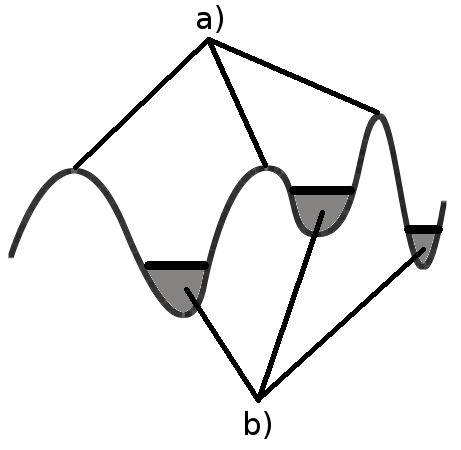
\includegraphics[width=9cm]{img/watershed-graphic}
  \caption{Graficzna reprezentacja a) wododziałów, b) zlewisk }
  \label{fig:watershed_graphic}
\end{figure}
W kontekście przetwarzania obrazów, wysokość terenu reprezentowana jest przez funkcję amplitudy gradientu obrazu lub funkcję intensywności obrazu, natomiast wododziały to ekstrema lokalne tych funkcji.
\subsubsection{Algorytm segmentacji wododziałowej}
Omawiany niżej algorytm został zaproponowany przez F. Meyera.
\begin{enumerate}
  \item wybierane są punkty startowe, będące również etykietami poszczególnych segmentów obrazu,
  \item sąsiadujące z wybranymi w kroku 1) punktami piksele umieszczane są w kolejce priorytetowej, gdzie priorytet stanowi jasność piksela,
  \item z kolejki pobierany jest piksel o najwyższym priorytecie. Jeśli wszystkie piksele w jego sąsiedztwie, którym została przypisana etykieta, mają tę samą etykietę, wtedy przetwarzany piksel również otrzymuje tę etykietę,
  \item wszystkie sąsiadujące piksele, które nie zostały oznaczone etykietą, umieszczane są w kolejce,
  \item jeśli kolejka nie jest pusta, powtarzany jest punkt 3). W przeciwnym razie algorytm zostaje zakończony.
\end{enumerate}
Piksele, które nie zostały oznaczone, reprezentują wododziały. Piksele oznaczone tą samą etykietą, należą do tego samego zlewiska, czyli tworzą ten sam segment.
